Hacer que las aplicaciones de Node.js estén listas para producción es probablemente el tema más oculto y omitido en la literatura de Node.js, pero es uno de los más importantes \cite{mardan}. Se requiere de un método estandarizado para que la efectividad del despliegue en el servidor de producción sea optima.

\subsubsection{Requisitos del servidor}

\begin{itemize}
  \item Servidor CentOS 7 con Node.js y Git instalado.
  \item Al menos 512 Mb de RAM y 15 Gb de espacio libre en disco.
  \item Acceso de usuario root a través de SSH.
  \item Un nombre de dominio apuntado a la dirección IP del servidor (rosesland.app)
  % \item Editor de texto nano, puede instalarse con este comando:\\
  
  % \code{yum install nano}
\end{itemize}

\subsubsection{Servidor Privado Virtual}
Esta tecnología permite ejecutar las instancias de múltiples servidores en un servidor host físico de forma segura. Es un tipo de servidor de alojamiento web donde el alojamiento generalmente se realiza dividiendo un servidor físico principal en diferentes servidores virtuales múltiples. Cada uno de los servidores del sistema obtiene su propia parte de los recursos en función de los requisitos del cliente.
\vspace{0.8cm}

Este proyecto utiliza un servidor privado virtual (VPS) alojado en Digital Ocean, en donde debe decidir qué sistema operativo se desea, configurar el acceso SSH, crear un firewall, instalar los distintos lenguajes que necesita, etcétera. Para crear el VPS para el proyecto se accede a www.digitalocean.com y se crea una cuenta en Digital Ocean. Es necesario verificar la cuenta con una dirección de correo electrónico antes de poder crear un proyecto. Una vez verificada la dirección de correo electrónico, deberá un método de pago para el servicio. Al finalizar el registro y el modo de financiamiento se puede comenzar a configurar un servidor o Droplet. En Digital Ocean un Droplet es una máquina virtual simple y escalable. Con un costo de solo 5 dolares al mes, el plan básico es lo suficiente para mantener el proyecto en operación.
\vspace{0.8cm}

\begin{figure}[H]
  \centering
  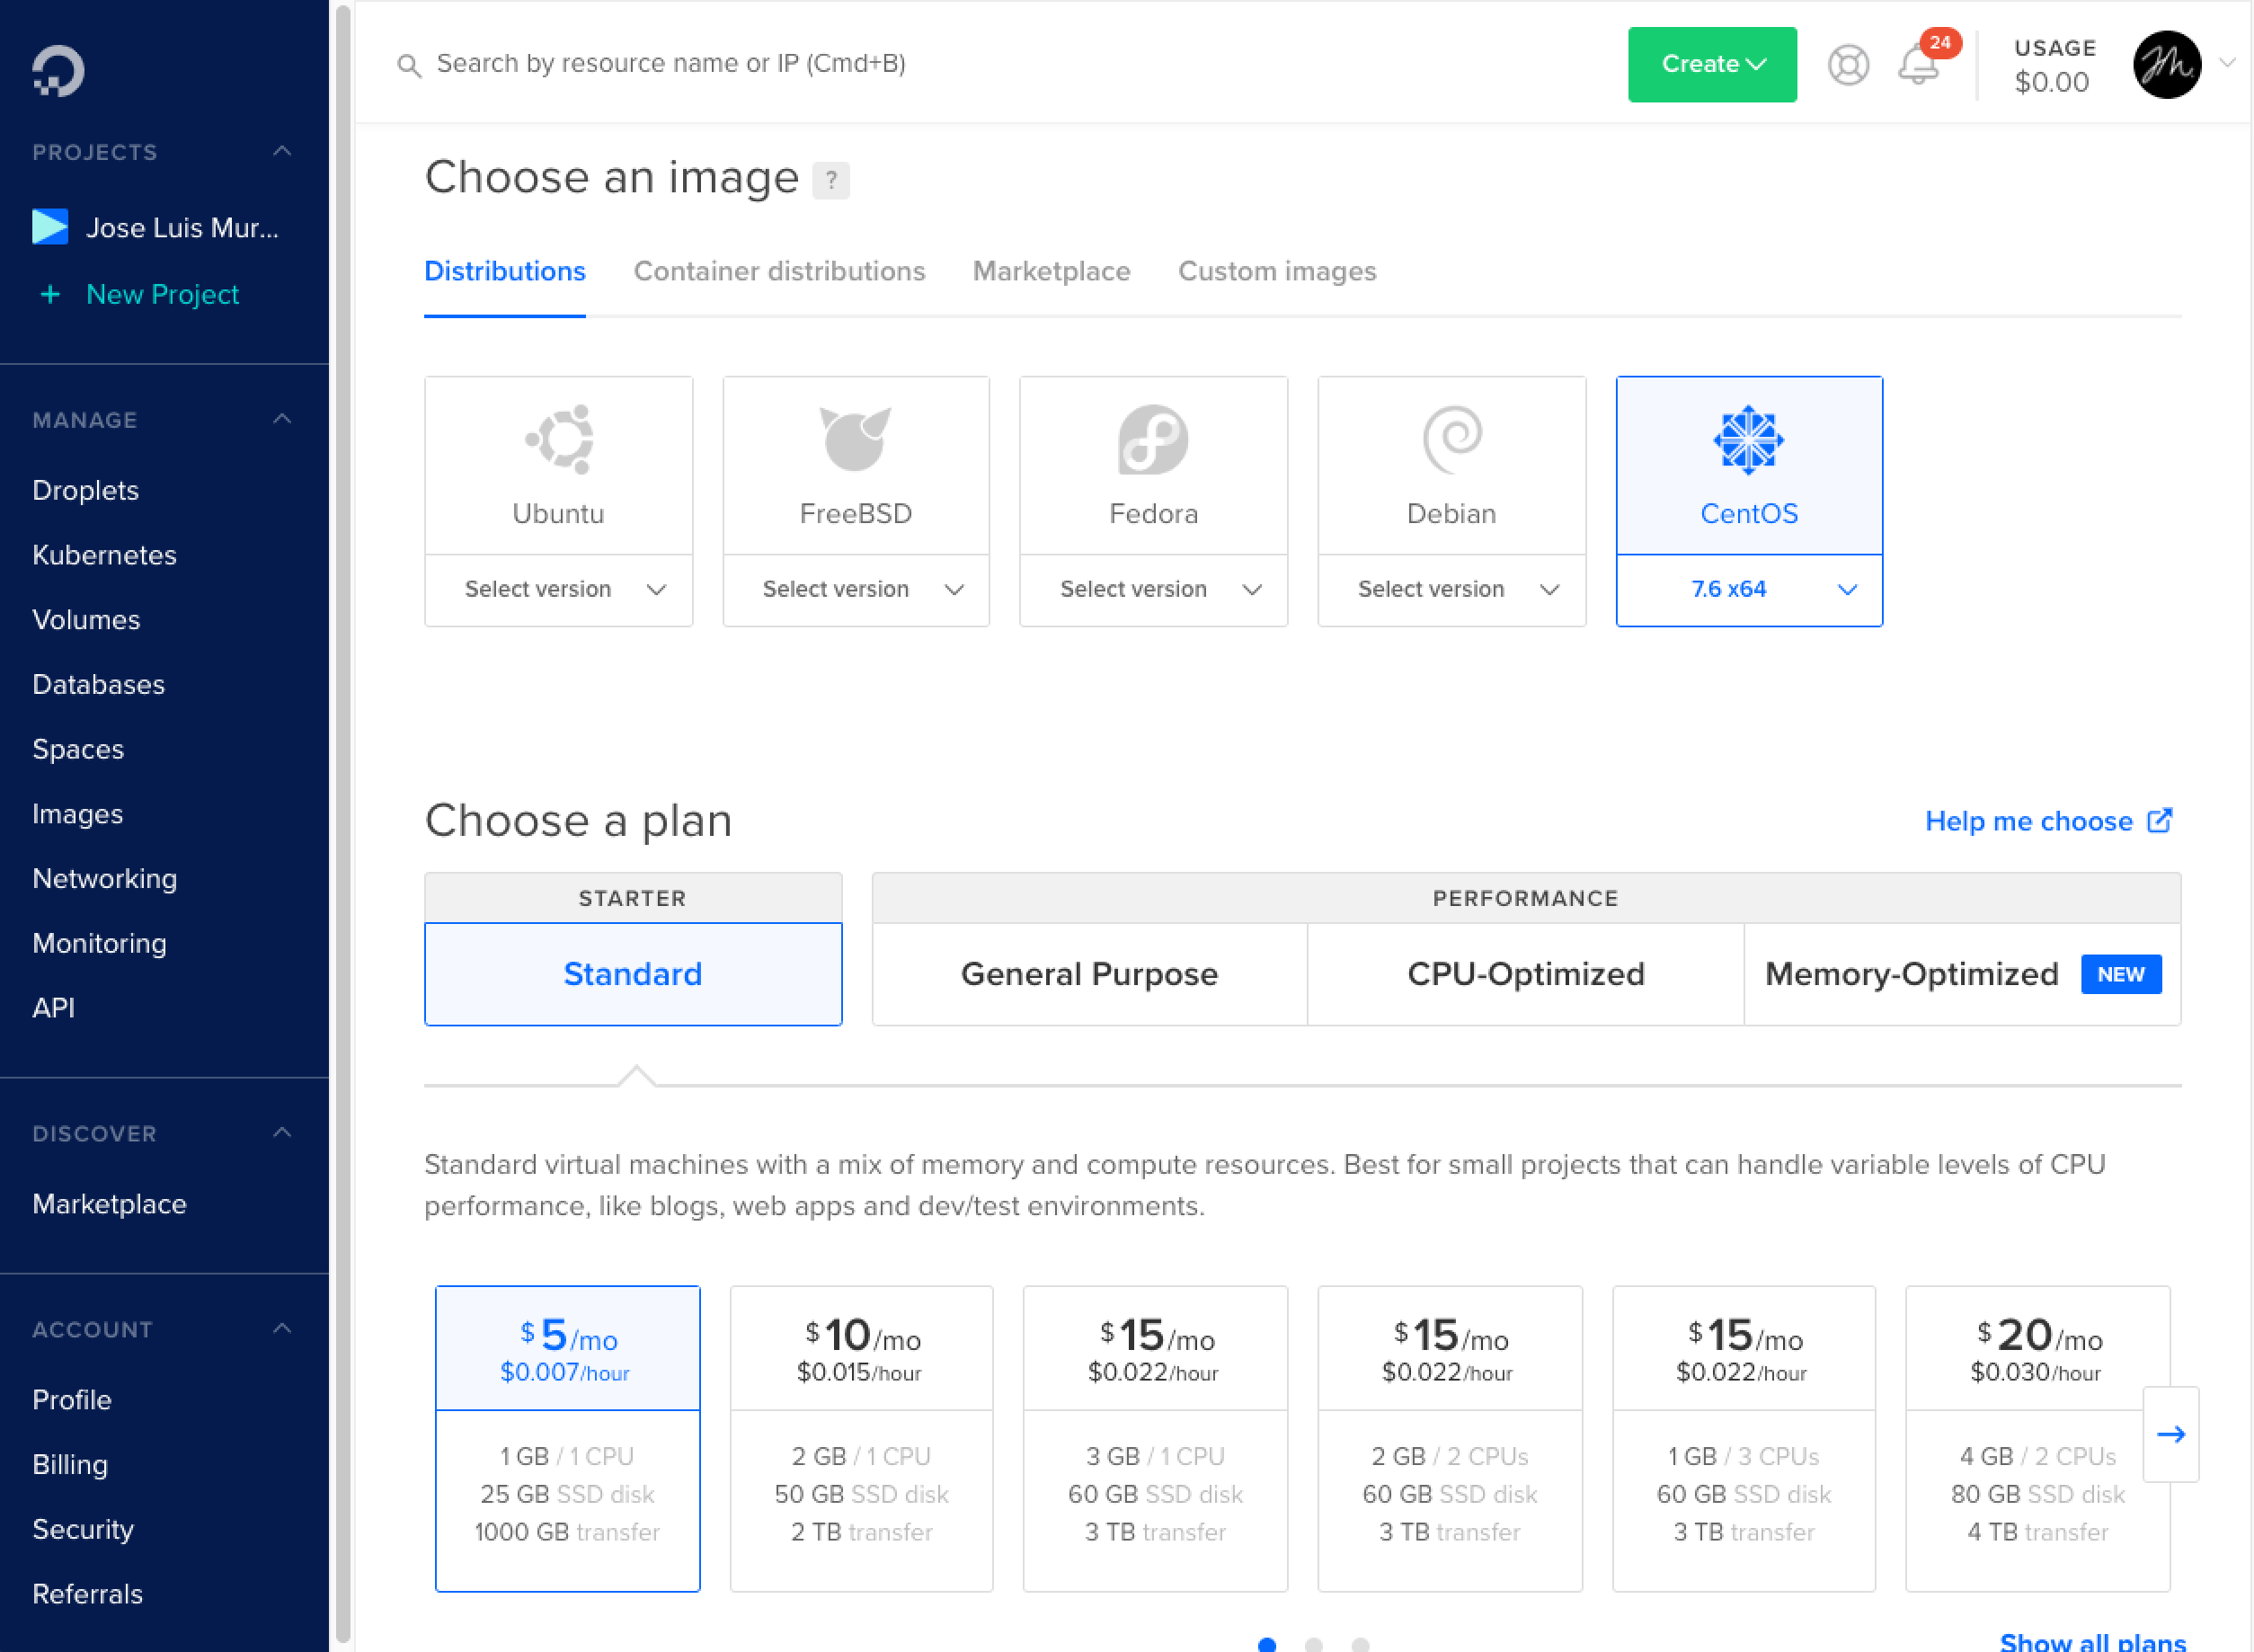
\includegraphics[width=1\textwidth]{digital-ocean}
  \caption{Configuración básica del servidor virtual privado.}
  \label{digital-ocean}
\end{figure}

Una vez que el servidor es creado, se recibe un correo electrónico de Digital Ocean. Este correo electrónico contiene los detalles de inicio de sesión para el servidor, en donde podremos conectarnos mediante SSH.
\vspace{0.8cm}

\subsection{Configurar despliegue automático con Git}
Al utilizar Git, el flujo de trabajo generalmente se dirige solo al control de versiones. Se tiene un repositorio local donde se trabaja y un repositorio remoto donde se mantiene todo sincronizado y se puede trabajar con un equipo y diferentes máquinas. Pero también es posible usar Git para mover una aplicación a producción \cite{vaccaro}.
\vspace{0.8cm}

\subsubsection{Configuración de repositorios}
Para poder empujar cambios a nuestro repositorio remoto se debe establecer la siguiente estructura:

\begin{itemize}
  \item Directorio publico del servidor: /var/www/rosesland.app
  \item Directorio del repositorio del servidor: /var/repo/site.git
\end{itemize}

Se inicia sesión en el VPS desde la consola de comandos y se ingresa lo siguiente:\\
\\
\code{cd /var}\\
\code{mkdir repo \&\& cd repo}\\
\code{mkdir site.git \&\& cd site.git}\\
\code{git init ---bare}\\

\code{---bare} significa que la carpeta no tendrá archivos fuente, solo el control de versiones.

\subsubsection{Git Hooks}
Los repositorios de Git tienen una carpeta llamada \code{hooks}. Esta carpeta contiene algunos archivos de muestra para conectar y realizar acciones personalizadas. La documentación de Git define tres posibles enlaces de servidor: \textit{pre-recepción}, \textit{post-recepción} y \textit{actualización}. Para este proyecto se necesita un `\gls{hook}' para post-recepción, que se ejecuta cuando un `envío' está completamente terminado.
\vspace{0.8cm}

En el repositorio se encuentran algunos archivos y carpetas, incluida la carpeta \code{hooks}. Se accede a ella mediante el siguiente comando.\\
\\
\code{cd hooks}\\
\\
Se crea el archivo post-recepción escribiendo:\\
\\
\code{cat > post-receive}\\
\\
Al ejecutar este comando, se muestra una línea en blanco que indica que todo lo que escriba se guardará en este archivo. Se debe agregar lo siguiente:\\
\\
\code{\#!/bin/sh}\\
\code{git --work-tree=/var/www/rosesland.app --git-dir=/var/repo/site.git checkout -f}\\
\\
Al terminar, se presiona `control-d' para guardar. Para ejecutar el archivo, se necesita establecer los permisos adecuados usando:\\
\\
\code{chmod +x post-receive}\\
\\
El archivo post-recepción se examina cada vez que se completa un envío y coloca los archivos en \code{/var/www/rosesland.app}, esto permite actualizaciones directas del proyecto facilitando el mantenimiento de codigo y evitando la tarea de tener que conectarse al servidor para cargar los archivos manualmente.
\vspace{0.8cm}

En el repositorio local se necesita configurar la ruta del repositorio remoto. Se le dice Git que agregue un control remoto llamado `live':\\
\\
\code{git remote add live ssh://root@rosesland.app/var/repo/site.git}\\
\\
Con esto es posible empujar cambios en el repositorio al servidor remoto usando el alias `live':\\
\\
\code{git push live master}\\
\\
Con esto se le dice a Git que empuje al remoto `live' en la rama `master'.
\vspace{0.8cm}

\subsection{Despliegue Node.js en un entorno de producción}
El término servidor puede ser un poco confuso para las personas nuevas en el tema porque puede referirse tanto al \gls{hardware} (computadoras físicas que albergan todos los archivos requeridos por los sitios web) como al \gls{software} (programa que permite a los usuarios acceder a esos archivos en la web). El \gls{hardware} se encuentra alojado en un servidor virtual privado, por tal motivo esta sección se centra en el lado del software.

\subsubsection{Servidor proxy inverso}
Una vez transferido el código del proyecto al servidor y configurar un entorno para la aplicación, es momento de configurar un servidor proxy inverso. Un servidor proxy es un servidor intermedio o intermediario que reenvía solicitudes de contenido de varios clientes a diferentes servidores a través de Internet. Un servidor proxy inverso es un tipo de servidor proxy que generalmente se encuentra detrás del firewall en una red privada y dirige las solicitudes de los clientes al servidor apropiado. Un proxy inverso proporciona un nivel adicional de abstracción y control para garantizar el flujo fluido del tráfico de red entre clientes y servidores.

\subsubsection{Configuración nginx y firewall-cmd}
Nginx (Engine X) es una de las mejores soluciones para configurar un servidor proxy inverso, con el será posible entregar contenido de forma rápida, confiable y segura. Hará que la aplicación sea accesible desde un navegador, y en caso de ejecutar varios sitios desde el mismo servidor, también podría funcionar como equilibrador de carga.
\vspace{0.8cm}

Después de iniciar sesión como usuario root, se agrega el repositorio CentOS 7 \acrshort{epel} y se instala nginx con los siguientes comandos:\\
\\
\code{yum install epel-release}\\
\code{yum install nginx}\\
\\
Se presiona ‘y’ dos veces para finalizar la instalación. Para inicializar el servicio nginx y este inicie con el arranque del servidor se introducen los siguientes comandos:\\
\\
\code{sudo systemctl enable nginx}\\
\code{sudo systemctl start nginx}\\
\\
A continuación se instala firewall-cmd, el front-end de línea de comandos para firewalld (\gls{daemon} firewalld), para CentOS. Admite IPv4 e IPv6, zonas de firewall, puentes y conjuntos de ip, registra paquetes denegados, carga automáticamente módulos de \gls{kernel}, entre otras cosas más. Se instala con el siguiente comando:\\
\\
\code{yum install firewalld}\\
\\
Ahora, se habilita para que se inicie automáticamente en el arranque del sistema y se observa su estado:\\
\\
\code{systemctl start firewalld}\\
\code{systemctl enable firewalld}\\
\code{systemctl status firewalld}\\
\\
En nginx para CentOS se necesita crear carpetas para sitios disponibles y habilitados. Se crean con los siguientes comandos:\\
\\
\code{mkdir /etc/nginx/sites-available}\\
\code{mkdir /etc/nginx/sites-enabled}\\
\\
Después se edita el archivo de configuración global de nginx:\\
\\
\code{nano /etc/nginx/nginx.conf}\\
\\
Se identifica la linea:\\
\\
\code{include /etc/nginx/conf.d/*.conf;}\\
\\
Se inserta lo siguiente:\\
\\
\code{include /etc/nginx/sites-enabled/*;}\\
\code{server\_names\_hash\_bucket\_size 64;}
\vspace{0.8cm}

\begin{lstlisting}[language=bash, caption=Fragmento de configuración nginx]
http {
  include       /etc/nginx/mime.types;
  default_type  application/octet-stream;

  log_format  main  '$remote_addr - $remote_user [$time_local] "$request" '
                    '$status $body_bytes_sent "$http_referer" '
                    '"$http_user_agent" "$http_x_forwarded_for"';
  access_log  /var/log/nginx/access.log  main;
  sendfile        on;
  keepalive_timeout  65;

  #Se agrega debajo de esta linea
  include /etc/nginx/conf.d/*.conf;
  include /etc/nginx/sites-enabled/*;
  server_names_hash_bucket_size 64;
}
\end{lstlisting}

Para finalizar se procede a utilizar el modulo npm llamado `nginx-generator' para generar los archivos que le indican a nginx que actúe como un proxy inverso. En la linea de comandos se escribe lo siguiente:\\
\\
\code{nginx-generator \symbol{92}}\\
\code{        ---name rosesland \symbol{92}}\\
\code{        ---domain http://rosesland.app \symbol{92}}\\
\code{        ---type proxy \symbol{92}}\\
\code{        ---var host=localhost \symbol{92}}\\
\code{        ---var port=3000 \symbol{92}}\\
\code{        /etc/nginx/sites-enabled/rosesland.app.conf}\\
\\
Este comando crea un archivo llamado \code{site\_nginx} y lo coloca dentro del directorio \code{/etc/nginx/sites-enabled/}. El archivo se puede observar con el siguiente comando:\\
\\
\code{sudo nano /etc/nginx/sites-enabled/rosesland.app.conf}\\
\\
Por ultimo se reinicia nginx:\\
\\
\code{systemctl restart nginx}

\subsubsection{Configuración del administrador de procesos PM2}
PM2 es un administrador de procesos de producción para aplicaciones basadas en Node.js. Con PM2, se pueden monitorear aplicaciones, su memoria y uso de CPU. También proporciona comandos fáciles para detener/iniciar/reiniciar todas las aplicaciones o aplicaciones individuales. Una vez que la aplicación se inicia a través de PM2, siempre se ejecutará después de que el sistema se bloquee o reinicie.
\vspace{0.8cm}

PM2 se instala mediante npm con el siguiente comando:\\
\\
\code{npm install pm2 -g}\\
\\
Una vez instalado sera posible ejecutar la aplicación con PM2:\\
\\
\code{pm2 start /var/www/rosesland.app/index.js ---name rosesland}\\

\begin{figure}[H]
  \centering
  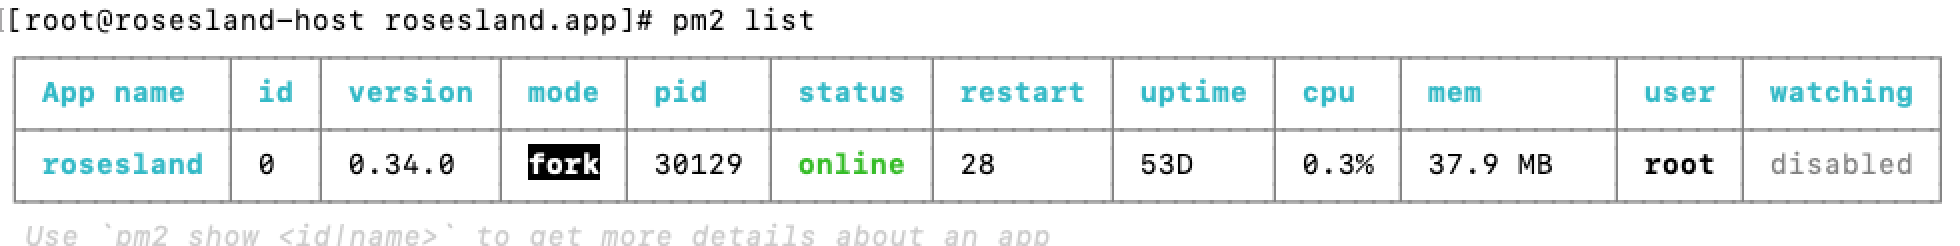
\includegraphics[width=1\textwidth]{pm2}
  \caption{Lista de procesos en pm2.}
\end{figure}

\subsubsection{Asegurar el sitio mediante HTTPS}
Con un nombre de dominio y registros DNS configurados correctamente para que apunten al VPS, se puede usar Certbot para generar certificados. Certbot es una herramienta de software gratuita y de código abierto para usar automáticamente certificados seguros en sitios web administrados manualmente para habilitar HTTPS \cite{certbot}.
\vspace{0.8cm}

Certbot está empaquetado en los Paquetes Adicionales para Enterprise Linux o EPEL (Extra Packages for Enterprise Linux). Para habilitar el repositorio adicional, el canal opcional e instalar EPEL, se emiten los siguientes comandos:\\
\\
\code{yum -y install yum-utils}\\
\code{yum-config-manager --enable \symbol{92}}\\
\code{rhui-REGION-rhel-server-extras rhui-REGION-rhel-server-optional}\\
\code{sudo yum install certbot python2-certbot-nginx}\\
\\
Se presiona `y' cuando es requerido y al finalizar ejecutamos certbot:\\
\\
\code{certbot --nginx}\\
\\
Cuando se instalan certificados por primera vez, Certbot pide una dirección de correo electrónico de emergencia, luego varias preguntas menos importantes y, finalmente, ¿desea redirigir todo el tráfico HTTP a HTTPS? Se selecciona la opción 2 para confirmar esta redirección y concluir con la configuración del despliegue de la aplicación.
\vspace{0.8cm}

En este momento se cuenta con una aplicación Node.js ejecutándose como un servicio en segundo plano en un entorno de producción, utilizando el protocolo HTTPS por seguridad y nginx como proxy inverso.
